% !TEX root = ../thesis.tex
\chapter{A Framework for Simulating and Analysing Cyber-Physical Systems}
\label{chap:framework}
% Describe what better CPS tools would provide - environmental simulation, trained environment models, virtual environments, cross-environment simulation
% Despite the growth in interest in the fields of sensor networks, cyber-physical computing and the Internet of Things, developing and testing sensor networks remains a difficult task, requiring developers to build reliable software which interacts as expected with the environment it inhabits.



% Testing and understanding how the environment interacts with a sensor network and vice-versa relies on placing the devices in the target environment and waiting for/creating the desired phenomena to interact with the network. Phenomena can include events such as movement of devices/objects, passive or active interaction with people (pressing buttons, triggering motion sensors), or other sensor events. Performing test deployments can be expensive, time-consuming and difficult.

% Existing tools and techniques aren't adequate for reliably and comprehensively testing these devices in the context of their target environment and the phenomena which may occur within it. Existing approaches for testing sensor networks have focused heavily on accurately simulating devices, the network and power consumption, with great success \cite{cooja, tossim}. However,  support for interacting with the environment is limited, typically performed using recorded or designed sensor trace data. This approach can be inaccurate, unrealistic and is restricted to what was recorded.


Despite the distributed and physical nature of cyber-physical systems and the Internet of Things, tools and techniques to support the needs of their development have not evolved to support efficient and reliable testing in the context of the deployment environment. Many tools exist which support individual aspects of testing and development, however, each one is siloed from the rest, limiting the overall ability and coverage of testing.

This chapter presents a CPS co-simulation framework designed to close the cyber-physical loop in CPS testing. Treating the physical environment as a first class citizen, the framework makes it possible for developers to simulate and test CPS within a 3D virtual environment, pre-deployment. A CPS interacts with and is directly affected by its target environment and inhabitants within it. The framework makes it easier for developers to test and analyse CPS which rely upon human mobility and device placement.

The following sections in this chapter outline a set of requirements \ref{sec:requirements} for the framework, a distributed design for building a co-simulation platform supporting plug-and-play of multiple tools, including a sensor network simulator and 3D game engine. Finally, we describe several case studies which are used to demonstrate and evaluate the co-simulation framework and its features.  


% Drill down into the perfect or ideal scenario, what we want to be able to do
% Sell each requirement, as if it is paramount
% Space(Placement), Time(control), People(Mobility)
\section{The Ideal System}
\label{sec:Requirements}
This section describes a key set of requirements that are necessary for a framework to support simulating and testing cyber-physical systems in virtual environments not only comprehensively and accurately, but also efficiently and effectively, such that developers benefit from using such a tool over simply testing in the real world or in a sensor network simulator.

Each of these requirements focus on key aspects needed for the framework to be effective for testing cyber-physical systems, which are deeply integrated into our physical world.

\subsection{Placement}
\label{sub:requirements_3D design and placement}
The issue of placement in CPS is tightly coupled to provisioning, i.e., what is the minimum number of devices needed and where should these devices then be placed in order to acheive the desired coverage, reliability, or other desired metric. 
Understanding how many devices are needed for a specific deployment and where to place them within the environment is a difficult challenge pre-deployment. Often based on guess-work, trial-and-error and field studies, which can lead to both over- and under-provisioning, resulting in either high-cost, a lack of network reliability, insufficient or redundant sensor data, etc. 
Thus, virtually experimenting with placement ahead of time will help mitigate these issues before deployment. 

Testing different placement strategies should be quick and efficient without the need to manually change scripts and sensor input traces; instead, the simulator should dynamically generate inputs for devices under test. Similarly, developers should be able to flexibly scale the levels of device provision, to test and understand how it will affect a deployment. Ideally, the system should support automatically testing and suggestion of optimum placement and provisioning levels, based of some selected criterion, such as cost, quality-of-service, robustness, etc.

\subsection{Phenomena-on-demand}
\label{sub:requirements_Phenomena-on-demand}
In order to test a CPS in the real-world, developers often need to wait for or force desired phenomena to occur in order to observe how the system reacts and whether or not it reacts correctly. However, exercising control over the real-world is a difficult and time-consuming challenge. Similarly, enlisting human participants to perform repetitive mundane tasks, requires paperwork, significant time and often money. Lastly, some scenarios are simply not feasible to test due to their scale, a deployment environment's limited access or health and safety concerns, e.g., outdoor environments, evacuation, fire, flooding.

Ideally, the framework should provide a dynamic and flexible method to create and/or script phenomena which interact with the system on demand. Unlike traces, a scripted phenomena, such as a person walking down a corridor, only needs to be updated once to change path with the virtual world dynamically generates sensor input, whereas, multiple traces feeding sensors simulated ``detections'' inputs need to be updated for each sensor device in the person's path, a time-consuming and unscalable solution.

%%%%%%%%%%%%%%%%%%%%

\subsection{Human Mobility} % (fold)
\label{sub:requirements_mobility}
Existing tools support the concept of device mobility, updating a device's radio model based on its location. However, in these tools device mobility in is pre-determined; in other words, developers define mobility patterns, as a sequence of positions, manually, which the network of devices must follow, but don't react to the live cyber-physical simulation. The tools have no concept of other entities, such as people, physical objects or gravity.

Because of the lack of support for simulating human mobility, developers are required to either manually trigger sensors or create custom mobility model scripts for each test scenario, in which the script triggers button presses or motion sensors at specific time intervals. As the network grows, shrinks or the layout changes, developers need to update the model for each device; this quickly becomes unmanageable as the network and number of tests scale in size.

Ideally, the framework should support testing CPS utilising real-time dynamic human (and device) mobility, enabling simulations to support testing environments in which virtual human participants interact with and are affected by the CPS and the environment, closing the cyber-physical loop. In other words, virtual participants are able to autonomously navigate an environment, based on flexible pre-assigned behaviours; including simple actions, such as patrol this corridor or walk to location A; or more complex behaviours, such as follow or avoid person X, wait on an event before moving. Whilst target locations may be pre-defined, routes may change in real-time based on obstacles or other behaviours. By combining behaviours, participants can dynamically generate phenomena for the CPS to sense and react to, in turn forcing the participants to react, and so on. 

Using such a system, when simulating a fire evacuation scenario, participants dynamically react to fire avoiding it as it spreads throughout the environment, with the CPS able to sense, alert and direct evacuees towards safe exits.

On top of this, it should also be possible to provide complex mobility and crowd behaviour, such that individual participants can be set to join and leave crowds of participants, moving as a unit through an environment.

% subsection mobility (end)


% Using Ard\'{a}n, developers can take direct control of a virtual person or script intelligent virtual crowds to carry out tasks, such as walking between points, avoidance, following or interacting with objects. Figure \ref{fig:views} shows people walking up and down a corridor, avoiding each other's path. Unlike using trace data, genuine or created, developers can easily tweak scenarios, such as moving sensors, people or adjusting behaviour, to test subtle or significant variations. Developers can also create scenarios that are difficult or dangerous to reproduce in the real world, such as emergency situations, and repeatedly test their applications without risk.

\subsection{Time Control}
\label{sub:requirements_Time Control}
In real-world deployments developers have no control over time and have to analyse events as they happen or rely on logs and video to record and view post-test. Simulation approaches enable pausing and slowing time, giving developers more time to analyse snapshots or small windows of time in a test, however, recording still utilises log-based approaches, providing only a limited snapshot. Both approaches provide limited views into a test, if events were not recorded, via logs, video or otherwise, they are lost and the test must be re-run.
Recording everything would enable a simulator to create a full reconstruction and allow developers to master time-control, moving forwards and backwards through a simulation to view its state at any point in time. Within a 3D environment, this would also allow developers to observe the context in which particular phenomena occur, enabling in-depth and contextual analysis.

Naturally, the system should support recording arbitrarily long, such as day- or even week-long, simulations, enabling longitudinal testing of CPS applications in real-time or faster. The system must also provide the means to quickly scrobble through recordings, based on time or checkpoints, generated based on points of interest.

\subsection{Distributed component-based simulation} % (fold)
\label{sub:distributed}
The co-simulator should be discretised into components with clear interfaces; such that the architecture allows for distributing components across multiple machines. Similarly, the architecture should support for allowing virtual components to be swapped out for other components, or their real counterparts e.g., swapping out a set of virtual simulated nodes for a set of real deployed hardware nodes.

% subsection distributed (end)
% Unlike in real world deployments, developers have the power to control time in the simulated world. Developers can: stop-the-clock, freezing both the simulation and world in time, whilst giving them full control over what they see, allowing more time to observe the environment and move between points of interest; slow down time, giving developers more time to observe or control the simulation; or even speed up time, providing desired results in considerably less time.


\subsection{Visualisation (Visual Diffing, Analytics)}
\label{sub:requirements_Visualisation}
To complement log output, existing CPS simulators provide basic visualisations, such as 2-dimensional network maps and transmission timelines, giving developers more insight into the network component in real-time. Many of these visualisations are transient and can only be viewed once as the simulation is on going. Thus, when trying to compare two separate simulation runs, developers still need to resort to post-simulation log analysis using external tools to manually process the log output, without the context of the simulation visualisation. 

When simulating in the context of a 3D virtual world, visualisations must add value to already busy simulations, with the aim to reduce the visual noise, not add to it. Thus, visualisations should not simply be added on top of the 3-dimensional virtual world, instead they should seamlessly integrate into the virtual environment to provide intuitive visual feedback, indicating points of interest, such that they further enhance a developers analytical tool-kit and understanding of an on-going simulation. 

Ideally, visualisations should help developers to spot and analyse differences between multiple runs in real-time, without the need the need to leave the tool to perform post-simulation data analysis using manual tools. These visual differencing tools, would allow developers to specify events of interest to watch, which the simulator then visually flags to the user when it happens, e.g., a node glows red when it's power levels drop below a certain point, or differ from a previous simulation run by x\%. Similarly, visualisations should also support longitudinal studies of systems.


% Ard\'{a}n provides developers tools to overlay visualisations of network and sensor meta-information on top of the virtual world to help understand how the network is running, allowing developers to see information such as how network paths form as packets are sent, as well as transmissions, receptions, interruptions. In figure \ref{fig:views}, sending devices are highlighted with a circle and receiving devices are connected by an arrow to the sender, each device is represented with its own colour, to help differentiate simultaneous transmissions.

\subsection{Virtual Sensors and Actuators}
\label{sub:requirements_Virtual Sensors and Actuators}
Sensor and actuator devices have both a hardware and software representation, thus, a framework must reflect both of these components within the simulated world. The CPS simulator runs the device program code, simulating the CPU, network and other virtual components, whilst within the game engine the device has a physical form with sensors and actuators that can perceive and interact with the virtual world. 

This will enable a co-simulation approach in which simulated hardware devices can interact directly with the 3D virtual environment, and not just with faked or simulated input from traces or user input. The framework will provide developers with flexible and dynamic environmental interaction between the CPS and the environment, closing the loop within a simulation. 

Visually, sensor hardware can be modelled at varying degrees of accuracy, depending on the requirements, e.g., virtual devices can be larger in size compared to real counter-parts, enabling easier location and observation. Similarly, sensing can be simulated to varying degrees of accuracy, again depending on the needs and simulation power available. 

% Within Ard\'{a}n we have modeled several basic sensors and actuators, including motion detectors, buttons, lights and location. These act as virtual hardware for the simulated sensors, allowing the simulation to interact with the virtual world. Virtual sensors can be designed to model a real sensors behaviour, or be virtually improved, providing higher accuracy or more features, not possible with existing hardware.

\subsection{Direct control}
\label{sub:requirements_direct_control}
The framework should allow direct control of three key aspects of the simulation: entities in the world, such as environmental attributes and physical devices or sensors; virtual people in the 3D world, enabling the developer to inhabit the world vicariously through a virtual person, interacting and responding to the world as if it were the real world; lastly, the view, allowing the developer to view the world from any angle at any point in time, including pausing the world mid-simulation and moving around, providing a better view of a point of interest.

\subsection{Write Once, Test Everywhere}
\label{sub:requirements_real_code}
Using a single language for both testing and deployment, in the real- and virtual-world, significantly reduces the time and effort for transferring between the different environments and ensures a consistent code-base, with the hope for consistent performance and output. Similarly, using an existing language reduces barrier to entry for use of a new tool and eliminates the opportunity for translation bugs being introduced when transitioning between test and deployment, whether they be real or virtual environments.

\subsection{Performance}
\label{sub:requirements_real-time_operation}
The system should support real-time operation so that simulations run as fast as, if not faster than their real counterparts, enabling quicker deploy-test-debug cycles. Similarly, it needs to be responsive to real-time direct interaction by developers, such that developers can observer, interact with and change ongoing simulations. Thus, in order for the framework to run in real-time, each of the components must also run accordingly. In order for the sensor network simulator to run in real-time, the 3D game engine must respond to all requests in real-time (sensor reads), such that the virtual hardware is in-discernible from the real counterpart.

\subsection{Synchronisation}
\label{sub:requirements_synchronisation}
Synchronisation, between the various components, including CPS simulator and 3D game engine clocks, ensures time sensitive events which rely on a global notion of time and delays occur correctly. Whilst real-time operation is also a requirement for all sub-systems, due to the differing simulation methods which aren't 100\% accurate and the intricacies of OS level scheduling, synchronisation is necessary to ensure that the individual sub-system's clocks stay in sync, within reasonable bounds. Similarly, communications between the sub-systems must be of low enough latency such that no additional delays are introduced. Typical applications are designed with predictable or known delays, such as opening a door after a motion event.

\subsection{Test cases}
\label{sub:requirements_test_cases} 
The system should provide support for automated testing, to observe and assert conditions about not only the CPS, but also the virtual world environment, akin to unit-testing available in traditional application development. Assertions would provide developers with warnings about phenomena that have occurred on a particular node, area, or within entire environment, such as ensuring a light's duty cycle doesn't exceed a set limit, checking a group of nodes are reporting similar information, or checking for network partitions once a node has moved out of an area.


\subsection{Modular environment building}
\label{sub:requirements_modular_building}
Designing 3D environments from scratch can be a slow and difficult process for non-expert 3D designers such as developers. Thus, in order to enable fast set-up, the system must support re-use and modification of existing pre-built environments and provide modular building blocks for building environments e.g., walls, doors, rooms, sensors, lights, agents.


% MOTHERHOODS - Scalable, extensibles, blah
\subsection{Scalability} % (fold)
\label{sub:requirements_scalability}
The scale of cyber physical systems can range significantly between self-contained deployments within a single room to ones which cover entire buildings, streets or even cities. Deployments could be internal, external or a mix, each of which may effect design decisions and issues that may arise. A simulation framework needs to be capable of supporting from 10s to 100s of devices. Similarly, the simulator must also be able to support rich environments, including complex layouts, large numbers of people to inhabit the world and environmental effects.
% subsection scalability (end)



\subsection{Extensibility} % (fold)
\label{sub:requirements_extensibility}
The framework design should facilitate seamless integration of new tools to supplement or replace the existing ones. This allows future developers to build upon and improve the co-simulation framework, its output and experience through the use of additional tools, including simulation tools, analytical tools, model checkers or real test-beds.

% % subsection extensibility (end)
% \textbf{Common Schema - }
% In order to ensure information communicated between individual sub-systems correspond, all information passed between the different tools must match or conform to a common schema, such as time, location and sensed units; without this conformity, even the simplest of interactions, such as device movement through a space, could be misunderstood between sub-systems, cm vs mm vs feet. This builds upon the extensibility requirement, ensuring future tools that support the schema will integrate seamlessly into the system.





% \textbf{Time control - }
% Whilst observing an ongoing simulation the developer should be able to pause the ongoing simulation allowing them to view a snapshot in time in more detail, both in terms of the running application and the 3D world, before resuming, speeding up or stepping through the simulation. Full control would allow the developer to also rewind back to an earlier state in the simulation and 3D world, enabling the developer to replay a set of events and observe multiple points of interest from different angles.





% \textbf{Scripted control - }
% Automated test cases are an important tool for testing systems repeatedly, thus, to support this the tool should allow developers to create scripted scenarios, in which people and objects within the 3D world can be instructed to follow set actions based on events, be it time, key presses or world events.



\section{Framework}
\label{sec:framework}
The current state-of-the-art for cyber-physical systems focuses on the network and hardware simulation components of testing, however, many other tools and platforms exist that could support other aspects of it, such as environment, physics, analysis without the need to directly extend or integrate these features directly within any of the existing tools. 
The goal of this framework is to provide a stable and extensible platform into which a variety of tools can be integrated into to support the simulation, testing, modelling and analysis of cyber-physical systems.

This section proposes an architecture for designing a distributed framework supporting the co-simulation and analysis of cyber-physical systems using multiple different tools.
This will enable information sharing between tools, enabling these tools to serve their purpose and close the loop, e.g., 3D simulator updates positions of devices based on physical interaction with the virtual world, this is then reflected in the network simulator which affects the radio transmission range and interference.



\subsection{Architecture} % (fold)
\label{sub:architecture}

% subsection architecture (end)
\begin{figure}[ht]
\centering
  % \includesvg[svgpath = ./imgs/, width = 0.5\textwidth]{architecture}
  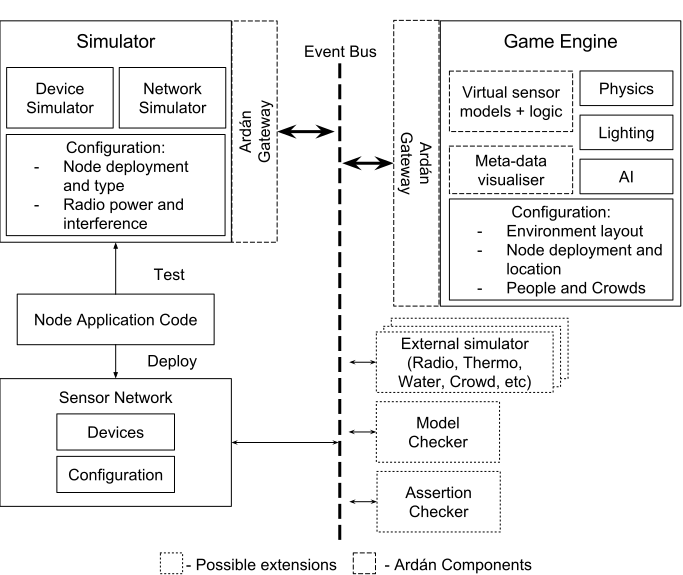
\includegraphics[width=0.5\textwidth]{./imgs/architecture}
  \caption{Ard\'{a}n architecture}
  \label{fig:architecture}
\end{figure}


Thus, rather than integrate the systems directly, our approach uses a pub-sub event bus and common schema to describe information passed between the different tools. This approach reduces the tight coupling between tools, allowing individual tools to be removed or new ones added with minimal configuration. We envision the use of tools such as model checking, statistical analysis, unit-testing and advanced simulation for radio and environmental properties.


\subsection{Communication Model} % (fold)
\label{sub:communication_model}

Discuss the use of a pub/sub for distributing simulation events and interactions between co-simulators.

\subsection{CPS Simulation} % (fold)
\label{sub:cps_simulation}
Discuss the use of the Cooja simulator to simulate C based sensor nodes using both emulation and simulation.
% subsection cps_simulation (end)

\subsection{Game Engine - Environment Simulation} % (fold)
\label{sub:environment_simulation}
Discuss the use of a modern game engine, Unreal Engine 4, to model and simulate a physical environment, including people.
% subsection environment_simulation (end)
% subsection communication_model (end)

\subsection{Time} % (fold)
\label{sub:time}
Describe the model of time and how different components coordinate.
% subsection time (end)